\documentclass[letterpaper,12pt]{texMemo}

\usepackage{indentfirst}
\usepackage{graphicx}
\usepackage{datetime}


%%===================== HEADER ====================================
\memoto{Bruce Bolden, Senior Instructor, University of Idaho}
\memofrom{Seth Forrest, Student, Java Group (\#3)}
\memosubject{ Progress Report - Goofy Glasses }
\memodate{\today}
%%=================================================================

\begin{document}
\maketitle

\section*{ Overview }

Most of the final sprint involved cleaning up the Grid Editor code base and a through cleaning of the documentation. There was a brief burst of work to prepare for the presentation of our editor, but after that our group decided that, for the most part, our program was complete, and the best use of the remaining time would be spent polishing the project instead of adding additional features.
\\
In addition to my organizational tasks, my role in this sprint, as in past sprints has been largely focused on the documentation end of things. I rewrote a large portion of the design document in preparation for submission. I also took charge of printing the hard-copy and organizing the binder.


\section*{ Appendices }

I have included a couple of screencaps that display my commit involvement in the GitHub repo, since I know of no better way to show my contribution.

\begin{figure}[h]
  \centering
  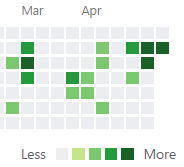
\includegraphics[width=.4\linewidth]{git_contrib} 
  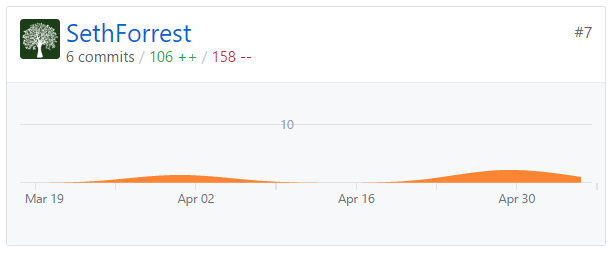
\includegraphics[width=.4\linewidth]{grid_commits}
  \caption{Spring Cleaning}
\end{figure}


\end{document}